% Created 2016-11-22 周二 18:27
\documentclass[journal]{IEEEtran}
\usepackage[utf8]{inputenc}
\usepackage[T1]{fontenc}
\usepackage{fixltx2e}
\usepackage{graphicx}
\usepackage{longtable}
\usepackage{float}
\usepackage{wrapfig}
\usepackage{rotating}
\usepackage[normalem]{ulem}
\usepackage{amsmath}
\usepackage{textcomp}
\usepackage{marvosym}
\usepackage{wasysym}
\usepackage{amssymb}
\usepackage{hyperref}
\tolerance=1000
\usepackage[thmmarks, amsmath, thref]{ntheorem}
\theoremstyle{definition}
\makeatletter \renewtheoremstyle{plain} {\item{\theorem@headerfont ##1\ ##2\theorem@separator}~}  {\item{\theorem@headerfont ##1\ ##2\ (##3)\theorem@separator}~}
\theoremheaderfont{\normalfont\bfseries}
\theoremseparator{:}
\theorembodyfont{\normalfont}
\theoremsymbol{\ensuremath{\blacksquare}}
\newtheorem{definition}{Definition}
\newtheorem*{proof}{Proof}
\newtheorem{prop}{Proposition}
\usepackage[caption=false,font=footnotesize]{subfig}
\usepackage{algorithm}
\usepackage{algpseudocode}
\renewcommand{\algorithmicrequire}{\textbf{Input:}}
\newcommand{\crhd}{\raisebox{.25ex}{$\rhd$}}
\renewcommand{\algorithmiccomment}[1]{{\hspace{-0.6cm}$\crhd$ {\it {#1}}}}
\interdisplaylinepenalty=2500
\date{}
\title{PCM Clustering based on Noise Level}
\hypersetup{
  pdfkeywords={},
  pdfsubject={},
  pdfcreator={Emacs 24.5.1 (Org mode 8.2.10)}}
\begin{document}

\maketitle
\begin{abstract}
Possibilistic c-means (PCM) based clustering algorithms are widely used in the literature. In this paper, we develop a noise level based PCM (NPCM) clustering algorithm. NPCM needs two kinds of information to specify for the clustering task, i.e., information of the cluster number and information of the property of clusters. More specifically, there are two parameters in NPCM where $m_{ini}$ is a possibly over-specified cluster number, and $\alpha$ characterizes the closeness of clusters in the clustering result. Furthermore, we find that the update of $\eta_j$ in adaptive PCM (APCM) is a positive feedback process and the adaptive $\sigma_v$ mechanism adopted in NPCM makes this positive feedback process more stronger, which leads to a faster convergence rate. Experiments show that the clustering result is not sensitive to the choosing of $\alpha$ unless there are overlapped clusters in the dataset.
\end{abstract}
\section{Introduction}
\label{sec-1}
The goal of clustering analysis is to discover natural groups of a set of points according to intrinsic characteristics or similarity \cite{jain_data_2010}. A fundamental question about clustering is how much information we should provide the clustering algorithm in order to discover natural (physical) clusters. K-Means \cite{jain_data_2010} and DBSCAN \cite{ester_density-based_1996} represent two different approaches. K-Means needs the exact number of clusters to work, whereas DBSCAN needs to know the lowest density (specified by two parameters: Eps and MinPts) for a cluster to form. K-Means needs only one parameter, but at the price of inability to handle noise and outliers, and the exact cluster number is very strong prior information. In contrast, DBSCAN provides the user much flexible in choosing parameters, and performs well in noisy environments.
Thus a good approach for a clustering algorithm may require two kinds of information, i.e., information of the cluster number and information of the property (e.g., density or closeness) of clusters.

Many clustering algorithms have the property that the cluster number is not needed to be exactly specified.
Although the approaches vary in certain aspects, a basic requirement is that information of the property of clusters should be sufficient to control the clustering process.
The CCM algorithm \cite{krishnapuram_fitting_1992} is run with a value that is higher than the number of physical clusters, then the algorithm merge the compatible clusters according to the compatibility conditions. The possibilistic c-means (PCM) \cite{krishnapuram_possibilistic_1993} algorithm also overcomes the need to specify the number of clusters and the power of PCM lie in finding meaningful clusters as defined by dense regions \cite{krishnapuram_possibilistic_1996}. The adaptive PCM (APCM) \cite{xenaki_novel_2016} algorithm makes PCM more flexible by adapting the bandwidth in each iteration. As seen from the above algorithms, reduced information of the cluster number is not sufficient for the clustering task. The CCM method needs to specify the compatibility conditions, i.e., information of when two clusters are compatible. PCM needs a reliable bandwidth (scale) estimate to function effectively. APCM adapts the bandwidth parameter in PCM but still needs to manually control the bandwidth by a parameter $\alpha$. The bandwidth in PCM and APCM is important information of the size of each cluster.

In the unified framework (UPCM) \cite{hou_pcm_2016} of PCM and APCM, the clustering process is analyzed from an uncertainty perspective, and the adaption of the bandwidth is performed in a more fuzzy way. There is also no need to specify the exact the cluster number in UPCM. There are three parameters to choose, i.e., the cluster number $m_{ini}$, the uncertainty of the estimated bandwidth $\sigma_v$, and the noise level parameter $\alpha$. However, the choosing of $\sigma_v$ depends on $\alpha$. In this paper, we aim to modify UPCM so that the information of the property of clusters is only characterized by one parameter, i.e., the noise level $\alpha$. 
The resulted algorithm is called the noise level based PCM (NPCM) clustering algorithm.

\textbf{Our Contributions:}
There are two parameters in NPCM: $m_{ini}$ is a possibly over-specified cluster number, and $\alpha$ characterizes the closeness of clusters in the clustering result.
Furthermore, we find that the update of $\eta_j$ is a positive feedback process and the adaptive $\sigma_v$ mechanism adopted in NPCM makes this positive feedback process more stronger, which leads to a faster convenience rate.
In addition, we address the background noise cluster problem encountered in APCM and UPCM to increase the algorithms' robustness in noisy environments.

\textbf{Related Works:}
Reducing the influence of points of other clusters on the $\boldsymbol{\theta}_j$ (prototype of cluster $C_j$) update is an important issue in the PCM literature, especially when there are close clusters in the dataset. One way to address this issue is to introduce sparsity on the membership values of a point by adding a penalty term of membership values (e.g., \cite{inokuchi_sparse_2007}\cite{xenaki_sparsity-aware_2016}) to the cost function, i.e., the membership of a point to a distant cluster is forced to be $0$. However, the modified cost function is difficult to solve. Another way to address the above issue is more direct. It is proposed in \cite{hou_pcm_2016} that each physical cluster can be seen as noise to other physical clusters, so a point is allowed to contribute to the adaption of $\boldsymbol{\theta}_j$ only if the membership value to cluster $C_j$ is larger than a threshold $\alpha$. The parameter $\alpha$ controls the closeness of clusters in the clustering result and is intuitive to choose. NPCM adopts the latter approach to represent the information of the property (closeness) of clusters via the parameter $\alpha$.

The rest of the paper is organized as follows. Section \ref{sec-2} introduces the background knowledge for our work. In Section \ref{sec-3}, the proposed noise level based PCM (NPCM) clustering algorithm is fully presented. In Section \ref{sec-4}, experiments are performed to illustrate the behavior of NPCM. Finally, concluding remarks are provided in Section \ref{sec-5}.
\section{Background Knowledge}
\label{sec-2}
In this section, we provide the background knowledge for our work. The PCM and APCM algorithms are first reviewed. Then, we review the UPCM algorithm, which utilizes the conditional fuzzy set framework to control the bandwidth of the membership function of points in a more natural and flexible way than APCM.
\subsection{The PCM and APCM Clustering Algorithms}
\label{sec-2-1}
The objective of possibilistic c-means (PCM) \cite{krishnapuram_possibilistic_1993} is to minimize the following cost:
\begin{equation}
J(\mathbf{\Theta},\mathbf{U})=\sum_{j=1}^{c}J_j=\sum_{j=1}^{c}\left[\sum_{i=1}^{N}u_{ij}d_{ij}^2+\gamma_j \sum_{i=1}^{N}f(u_{ij})\right]
\end{equation}
where $f(\cdot)$ can be chosen as:
\begin{equation}
f(u_{ij})=u_{ij}\log u_{ij}-u_{ij}
\end{equation}
$\mathbf{\Theta}=(\boldsymbol{\theta}_1,\ldots,\boldsymbol{\theta}_c)$ is a $c$-tuple of prototypes, $d_{ij}$ is the distance of feature point $\mathbf{x}_i$ to prototype $\boldsymbol{\theta}_j$, $N$ is the total number of feature vectors, $c$ is the number of clusters, and $\mathbf{U}=[u_{ij}]$ is a $N\times c$ matrix where $u_{ij}$ denotes the \emph{degree of compatibility} of $\mathbf{x}_i$ to the $j\text{th}$ cluster $C_j$ which is represented by $\boldsymbol{\theta}_j$. $\gamma_j$ can be seen as a bandwidth parameter of the possibility (membership) distribution for each cluster and is usually fixed in PCM based algorithms. Note that either $\gamma_j$ or $\sqrt{\gamma_j}$ can be referred to as the bandwidth for convenience in this paper.

Compared with fuzzy c-means (FCM) \cite{bezdek_pattern_2013}, PCM relaxes the constraint that the memberships of a datum to all clusters sum to $1$. So the generated memberships can be indicated as the typicality of a point to the cluster. This modification also leads to higher noise immunity with respect to FCM based algorithms \cite{barni_comments_1996}.

Minimizing $J(\mathbf{\Theta},\mathbf{U})$ with respect to $u_{ij}$ and $\boldsymbol{\theta}_j$ leads to the following two update equations:
\begin{IEEEeqnarray}{ll}
u_{ij}&=\exp\left(-\frac{d^2_{ij}}{\gamma_j}\right) \label{pcm_u_update}  \\
\boldsymbol{\theta}_j&=\frac{\Sigma_{i=1}^Nu_{ij}\mathbf{x}_i}{\Sigma_{i=1}^Nu_{ij}} \label{pcm_theta_update}
\end{IEEEeqnarray}

The major problem of PCM is that its performance relies heavily on good initial partitions and parameters \cite{nasraoui_improved_1996}. More specifically, the $c$ dense regions found may be coincident, as reported in \cite{barni_comments_1996}. Adaptive PCM (APCM) \cite{xenaki_novel_2016} solves this problem by adapting $\gamma_j$ at each iteration, and the clusters with $\gamma_j=0$ are eliminated. To handle the case where two physical clusters with very different variance are located very close to each other, APCM introduces a parameter $\alpha$ to manually scale the bandwidth:
\begin{equation}
\label{corrected_eta}
\gamma_j=\frac{\hat{\eta}}{\alpha}\eta_j
\end{equation}
where $\hat{\eta}$ is a constant defined as the minimum among all initial $\eta_j\text{s}$, $\hat{\eta}=\min_j\eta_j$, and $\alpha$ is chosen so that the quantity $\hat{\eta}/\alpha$ equals to the mean absolute deviation ($\eta_j$)  of the smallest physical cluster formed in the dataset.
$\eta_j$ is updated at each iteration as the \emph{mean absolute deviation} of the most compatible to cluster $C_j$ data points which form a set $A_j$, i.e., $A_j=\{\mathbf{x}_i|u_{ij}=\max_r u_{ir}\}$.
\begin{equation}
\label{apcm_eta_update}
\eta_j=\frac{1}{n_j}\sum_{\mathbf{x}_i\in A_j}||\mathbf{x}_i-\boldsymbol{\mu}_j||
\end{equation}
where $n_j$ and $\boldsymbol{\mu}_j$ are the number of points in $A_j$ and the mean vector of points in $A_j$ respectively.
\subsection{The Conditional Fuzzy Set and the UPCM Algorithm}
\label{sec-2-2}
According to Zadeh \cite{zadeh_concept_1975}, a type-2 fuzzy set (T2 FS) is a fuzzy set whose membership values are type-1 fuzzy sets on $[0,1]$. However, the conventional type-2 fuzzy set definition (e.g., \cite{mendel_type-2_2002}) makes T2 FS a complex subject. To simplify this problem, Li-Xin Wang \cite{wang_new_2016} proposes a conditional fuzzy set framework: a \emph{conditional fuzzy set}, denoted as $X|V$, is a fuzzy set with membership function $\mu_{X|V}(x|V)$ depending on the fuzzy set $V$ whose membership function is $\mu_V(v)$. The membership function $\mu_{X|V}(x|V)$ characterizes the \emph{primary fuzziness} while $\mu_V(v)$ characterizes the \emph{secondary fuzziness}. This framework provides a much more natural framework to model the dependence of one fuzziness (uncertainty) on another fuzziness than the type-2 fuzzy set formulation \cite{wang_new_2016}.

A related concept is the marginal fuzzy set of $X|V$, denoted as $X$, which is a type-1 fuzzy set whose membership function $\mu_X(x)$ is determined through Zadeh's Compositional Rule of Inference:
\begin{equation}
\label{marginal_fs}
\mu_X(x)=\max_{v\in\Omega_V}\min[\mu_{X|V}(x|v),\mu_V(v)]
\end{equation}
Then the basic philosophy to deal with type-2 fuzziness is to use \eqref{marginal_fs} to "cancel out" the secondary fuzziness $V$ and transform the type-2 problems back to the ordinary type-1 framework. We can explicitly model the uncertainty of the membership caused by some parameter $V$ and "cancel" $V$ to get the type-1 marginal fuzzy set. Then the effect of the uncertainty of $V$ is incorporated into type-1 marginal fuzzy set.
Illustration for the incorporation of uncertainty can be referred to the example in \cite{hou_pcm_2016}.

The unified framework (UPCM \cite{hou_pcm_2016}) of PCM and APCM utilizes the conditional fuzzy set to incorporate fuzziness (uncertainty) of the estimated bandwidth to the fuzziness of the membership function of points. Specifically, the update of the membership function \eqref{pcm_theta_update} is modified as follows:
\begin{equation}
\label{upcm_u_update}
\mu_{ij}=\exp\left(-\frac{d_{ij}^2}{\gamma_j}\right)
\end{equation}
where $\gamma_j=\left(0.5\eta_{j}+0.5\sqrt{\eta_{j}^{2}+4\sigma_vd_{ij}}\right)^2$ and $d_{ij}=||\mathbf{x}_i-\boldsymbol{\theta}_j||$.
The bandwidth correction of \eqref{upcm_u_update} is more natural and flexible than that of that of \eqref{corrected_eta}.
Another feature of UPCM is that UPCM introduces the concept of \emph{noise level} $\alpha$ of the data set in the update equation of prototypes:
\begin{equation}
\label{upcm_theta_update}
\boldsymbol{\theta}_j=\frac{\Sigma_{i=1}^Nu_{ij}\mathbf{x}_i}{\Sigma_{i=1}^Nu_{ij}} \quad \text{for}\;u_{ij}\geq \alpha.
\end{equation}
By setting an appropriate $\alpha$, the influence of points in other clusters $\boldsymbol{\theta}_{i\neq j}$ on the $\boldsymbol{\theta}_j$ update is reduced. This feature allows us to control the closeness of clusters in the clustering result.
\section{Our Algorithm}
\label{sec-3}
In this section, we first present motivations of proposed noise level based PCM (NPCM) clustering algorithm, which is developed based on UPCM and APCM. To address the issue of background noise clusters, we propose to eliminate low-density clusters in the initial partition. Then, we cancel out the parameter $\sigma_v$ in UPCM by utilizing the interplay between $\alpha$ and $\sigma_v$. Finally, we analyze the benefit and the problem after adopting the adaptive $\sigma_v$ approach in NPCM, and summarize NPCM in Algorithm \ref{alg:npcm}.
\subsection{Motivations}
\label{sec-3-1}
There are two needs originated from APCM and UPCM to be addressed.
\begin{enumerate}
\item The performance of clustering algorithms should be robust to background noise. We find that both APCM and UPCM suffer from the problem of background noise clusters, i.e., the background noise clusters are highly possible to become very large. So the physical clusters can't be correctly discovered. See Fig.\ref{fig_background_noise} for illustration.
\item The clustering algorithms should have as less parameters as possible, and the parameters should be intuitive to choose. APCM exerts strong control over the bandwidth correction process, i.e., the estimated bandwidth is directly scaled by the user-specified parameter $\alpha$ which is difficult to choose basing on intuition. In order to correct the bandwidth in a more fuzzy way, UPCM introduces an uncertainty parameter $\sigma_v$ to regulate the shape of the membership function. However, choosing $\sigma_v$ depends on the noise level parameter $\alpha$. The experiments in \cite{hou_pcm_2016} suggest that a small $\alpha$ should correspond to a small $\sigma_v$, and a large $\alpha$ to a large $\sigma_v$. So we can exploit this intuition to cancel out the parameter $\sigma_v$.
\end{enumerate}
\begin{figure}[tb]
\captionsetup[subfloat]{farskip=1pt,captionskip=1pt}% use this to reduce space between rows of subfloats, or between subfloat and the caption
   \centering
   \subfloat[]
    {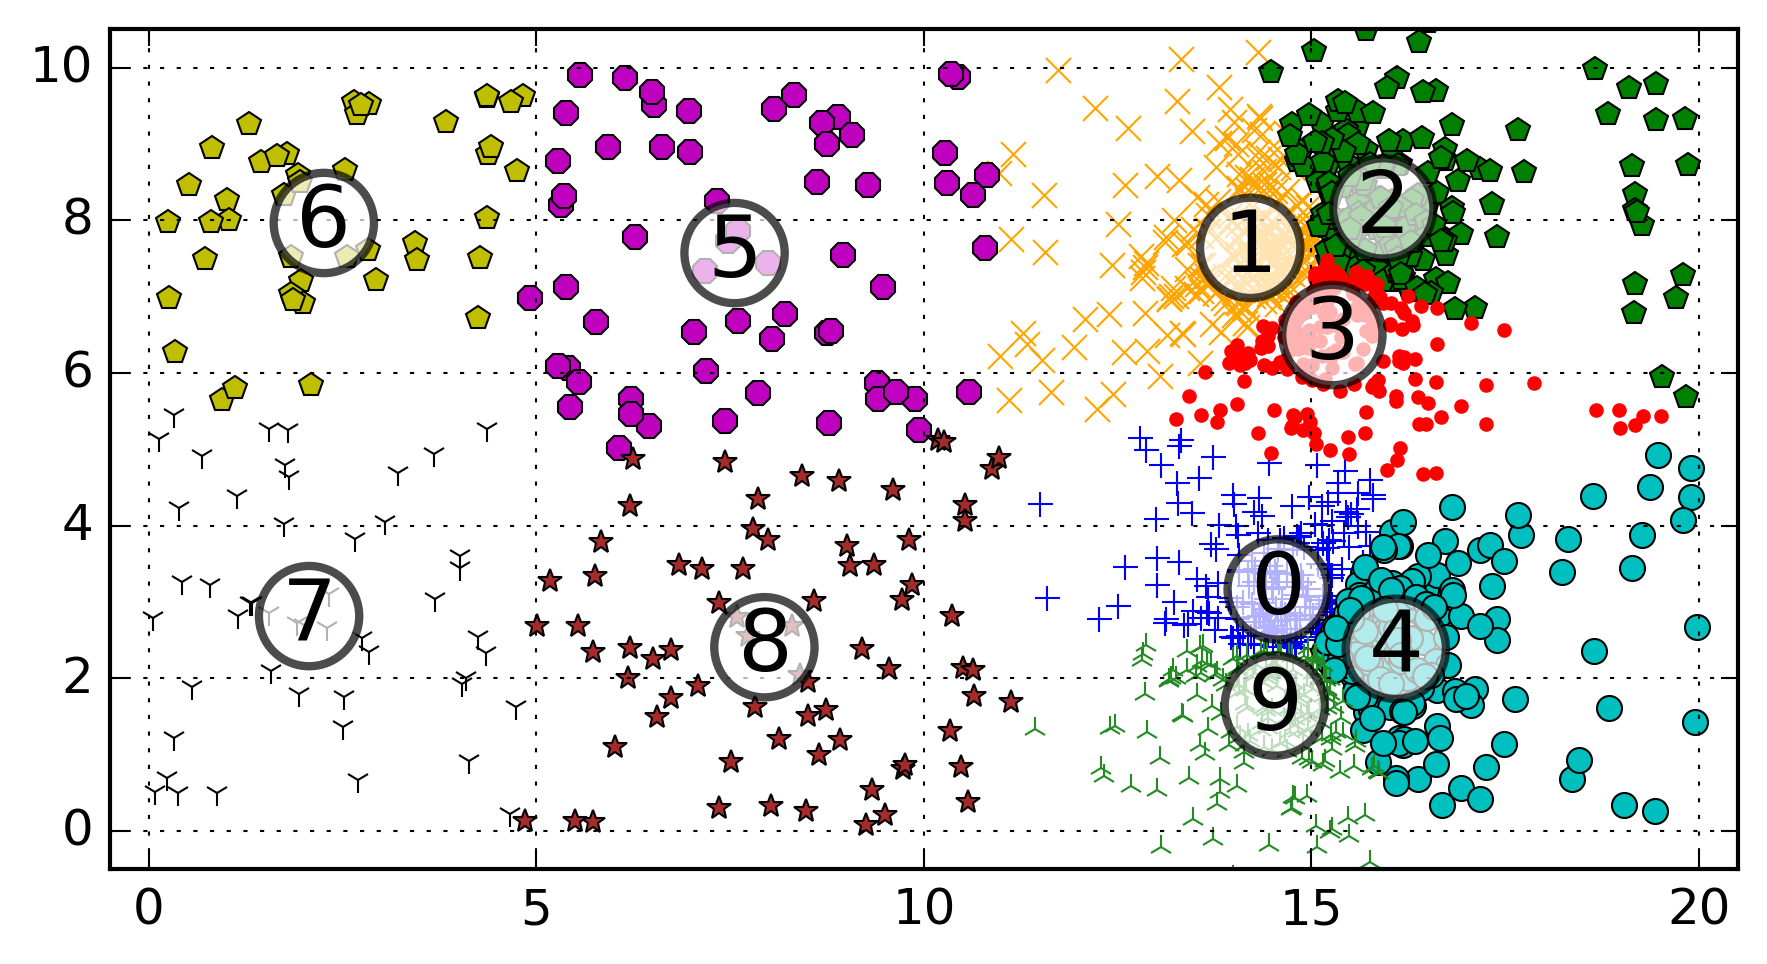
\includegraphics[width=\columnwidth]{img/noise_cluster_problem_ini.png}\label{fig_sub_noise_ini}} \\
   %\quad
   \subfloat[]
    {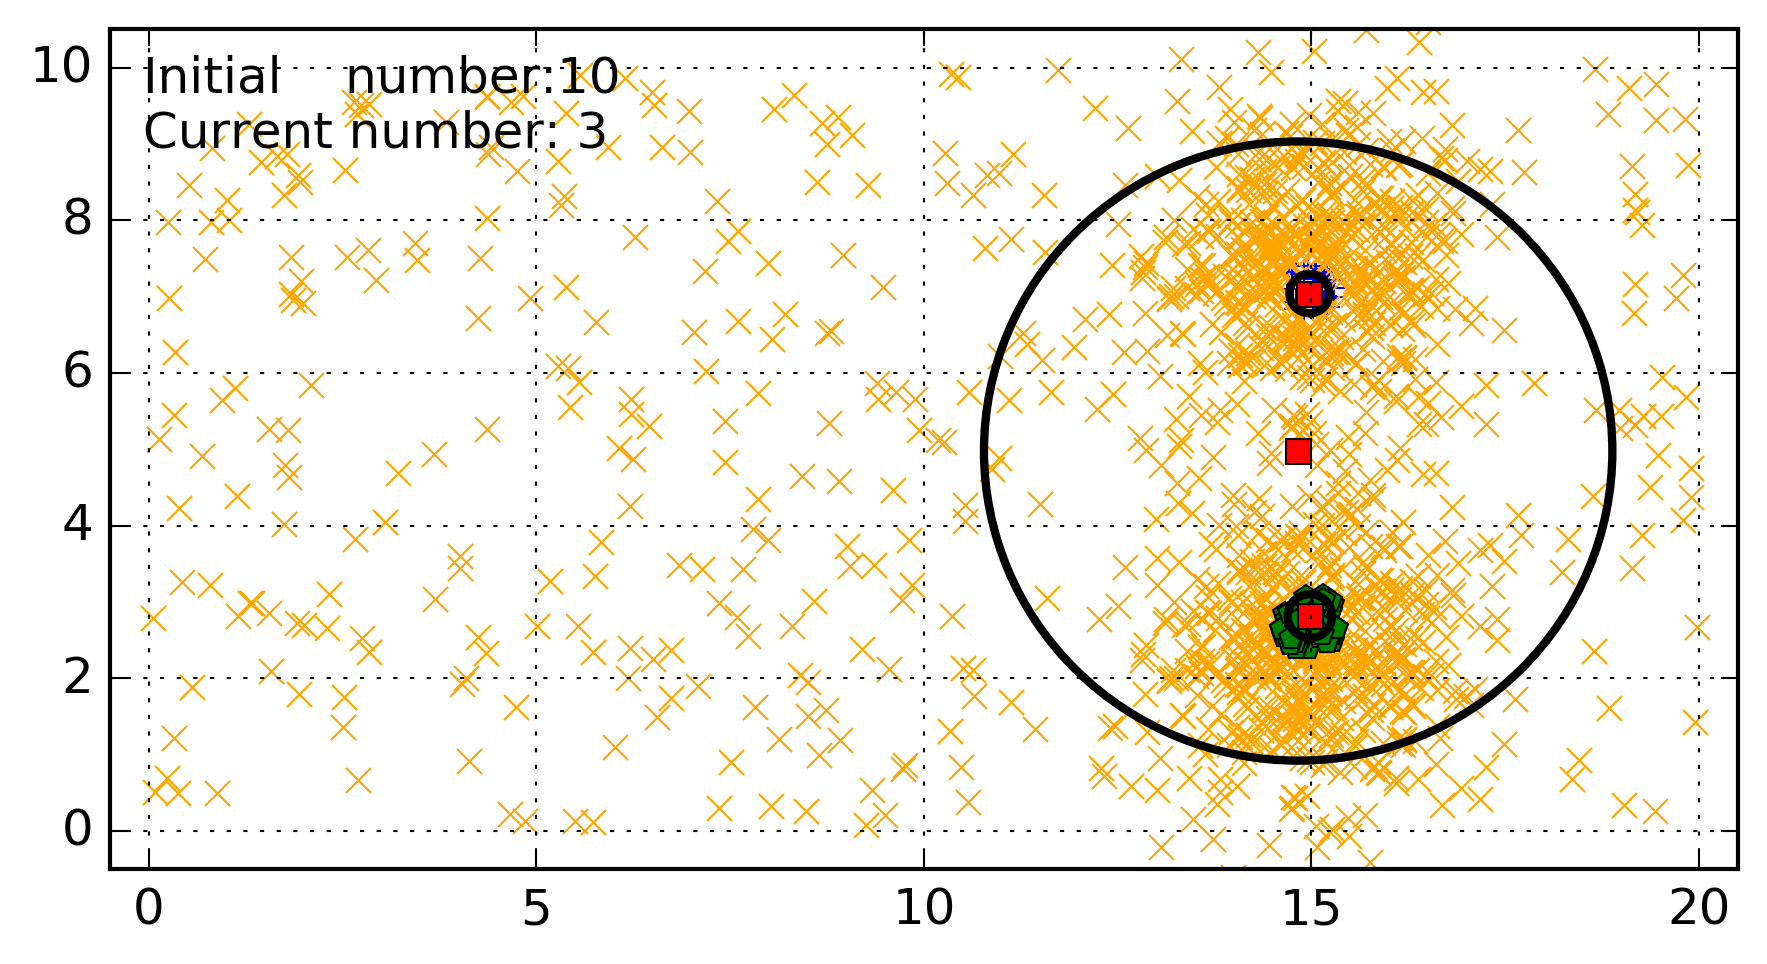
\includegraphics[width=\columnwidth]{img/noise_cluster_problem_last_frame.png}\label{fig_sub_noise_result}}
\caption{(a) 10 initial partitions obtained by FCM. (b) This clustering result can be generated by running UPCM with $\alpha=0$, $\sigma_v=1$, or by running APCM with $\alpha=0.5$ }
\label{fig_background_noise}
\end{figure}
\subsection{Initialization in NPCM}
\label{sec-3-2}
There are two issues with the initialization of NPCM. First, as in APCM and UPCM, NPCM needs an over-specified number of clusters $m_{ini}$ of the true number of clusters $m$. In the initial partition of the dataset, there should be at least one cluster placed near each physical cluster. 
It's shown in \cite{panda_comparing_2012} that K-Means is faster than FCM. So we choose K-Means to get the initial partitions of the dataset. Let $A_j^{ini}$ be the set of points $\mathbf{x}_i$ that belong to cluster $C_j$ and $n_j$ be the size of $A_j^{ini}$. Then the we set
\begin{IEEEeqnarray}{ll}
\boldsymbol{\theta}_j &= \frac{\Sigma_{i}\mathbf{x}_i}{n_j}  \quad \text{for}\;\mathbf{x}_i \in A_j^{ini} \label{npcm_ini_theta}\\
\eta_j &= \frac{1}{n_j}\sum_{\mathbf{x}_i \in A_j^{ini}}||\mathbf{x}_i-\boldsymbol{\theta}_j|| \label{npcm_ini_eta}
\end{IEEEeqnarray}
Second, as stated in the motivations, the background noise clusters in the initial partition should be eliminated. To address this issue, we define the density of a cluster as:
\begin{equation}
\label{npcm_density}
\rho_j=\frac{n_j}{\eta_j^d}
\end{equation}
where $d$ is the dimension of $\mathbf{x}_i$. Let $\rho_0=\max_j\rho_j$. Then cluster $C_j$ is a noise cluster and is eliminated if $\rho_j<0.1\rho_0$. For the case of Fig.\ref{fig_sub_noise_ini}, clusters 5, 6, 7, and 8 will be eliminated.
\subsection{Modeling the Relation Between $\alpha$ and $\sigma_v$}
\label{sec-3-3}
In UPCM, the noise level parameter $\alpha$ is introduced to reduce the influence of points in other clusters $\boldsymbol{\theta}_{i\neq j}$ on the $\boldsymbol{\theta}_j$ update. Specifically, $\alpha$ measures the closeness of two cluster prototypes in the clustering result. When a large $\alpha$ is specified, we consider that there may be clusters very close to each other, and the $\eta_j$ estimated in this case may be very uncertain. With the above interpretation of $\alpha$, the interplay between $\alpha$ and $\sigma_v$ becomes simple and intuitive, i.e., a large specification of noise level $\alpha$ means that few points (that we consider as good points) actually contribute to the adaption of prototype $\boldsymbol{\theta}_j$, so we should specify a large $\sigma_v$ to give the clusters in one physical cluster more mobility
\footnote{From \eqref{upcm_u_update}, we see that increasing $\sigma_v$ can increase $u_{ij}$ of a point $\mathbf{x}_i$, and from \eqref{upcm_theta_update}, we see that cluster $C_j$ moves (i.e., change of $\boldsymbol{\theta}_j$) only when there are enough points that meet the condition $u_{ij}\geq \alpha$.}
to merge; on the other hand, a small specification of $\alpha$ means that we are less uncertain about the estimated bandwidth, and more points are contributed to the adaption of $\boldsymbol{\theta}_j$, so we should also specify a small $\sigma_v$ \cite{hou_pcm_2016}. 

Before proceeding, we take a look at the the role of $\sigma_v$ in the clustering process of UPCM. UPCM exploits the conditional fuzzy set to incorporate the uncertainty of the estimated bandwidth. As can be seen from \eqref{upcm_u_update}, the actual bandwidth of the membership function $u_{ij}$ varies according to $\sigma_v$ and $d_{ij}$. In other words, the shape of the membership function becomes flatter when $\sigma_v$ or $d_{ij}$ increases. Note that a larger bandwidth corresponds a flatter membership curve. This observation suggests that the bandwidth itself can indicate the uncertainty of the estimated bandwidth, i.e., a large estimated bandwidth should correspond to a large $\sigma_v$. We will see that the formulation of NPCM meets this requirement.

From \eqref{upcm_u_update}, we can calculate the distance $d_{j\alpha}$ beyond which a point can't be used to contribute to the adaption of cluster $C_j$ by letting
\begin{equation}
\exp\left(-\frac{(d_{j\alpha})^2}{\gamma_j}\right)=\alpha,
\end{equation}
which leads to
\begin{equation}
\label{npcm_d_alpha}
d_{j\alpha}=\sqrt{-\ln\alpha}\left(\eta_j+\sqrt{-\ln\alpha}\sigma_v\right)
\end{equation}

When there is no uncertainty in the estimated bandwidth, we get $d_{j\alpha}^0=\sqrt{-\ln\alpha}\eta_j$. For a fixed $\alpha$, a large $\sigma_v$ will cause $d_{j\alpha}$ to become larger, which reduces the effect of $\alpha$ (see \eqref{upcm_theta_update}). This observation, together with the intuitive interplay between $\alpha$ and $\sigma_v$ we get from UPCM, suggests that we can explicitly specify a relation between $\alpha$ and $\sigma_v$. More specifically, we define the effect of $\sigma_v$ as the correction of $d_{j\alpha}^0$ by considering the uncertainty of the estimated bandwidth:
\begin{equation}
\frac{d_{j\alpha}-d_{j\alpha}^0}{d_{j\alpha}^0}=\frac{\sqrt{-\ln\alpha}\sigma_v}{\eta_j}=0.2,
\end{equation}
which leads to 
\begin{equation}
\label{npcm_sig_alpha_relation}
\sigma_v=0.2\frac{\eta_j}{\sqrt{-\ln\alpha}}
\end{equation}
Note that we can choose a value that is not 0.2 in the above formulation. From \eqref{npcm_sig_alpha_relation}, we can see that the cluster with large $\eta_j$ has a large bandwidth estimation uncertainty $\sigma_v$. The update of the membership function is modified according to \eqref{upcm_u_update} and \eqref{npcm_sig_alpha_relation} as:
\begin{equation}
\label{npcm_u_update}
\mu_{ij}=\exp\left(-\frac{d_{ij}^2}{\gamma_j}\right)
\end{equation}
where $\gamma_j=\left(0.5\eta_{j}+0.5\sqrt{\eta_{j}^{2}+0.8d_{ij}\eta_j/\sqrt{-\ln\alpha}}\right)^2$ and $d_{ij}=||\mathbf{x}_i-\boldsymbol{\theta}_j||$.
\subsection{Adaption of $\eta_j$ and the Algorithm Description}
\label{sec-3-4}
The update mechanism of $\eta_j$ in APCM and UPCM, that only data points that are most compatible to cluster $C_j$ can be used to update $\eta_j$ (see \eqref{apcm_eta_update}), makes the adaption of $\eta_j$ a positive feedback process. More specifically, if $\eta_j$ is large, then there may be more points to compute $\eta_j$ in the next iteration, which leads $\eta_j$ to become larger.
The benefit of the above positive feedback process is that the generated $\eta_j$ can automatically adapt to fit the corresponding physical cluster after convergence is reached.
Note that there is at most one cluster in each physical cluster when convergence is reached (the proof for cluster elimination and convergence of the prototypes to the center of dense regions in NPCM is given in the Appendix).

The difference between NPCM and the previous algorithms (i.e., APCM and UPCM) is that the introduction of adaptive $\sigma_v$ makes the positive feedback process more stronger 
\footnote{For the same $\eta_j$, a larger $\sigma_v$ means that the point $\mathbf{x}_i$ with distance $d_{ij}$ to cluster $C_j$ now has a larger $u_{ij}$, which can be seen from \eqref{upcm_u_update}. As a result, $\mathbf{x}_i$ with large $d_{ij}$ can be more compatible to cluster $C_j$ in the next iteration, so the adjustment of $\eta_j$ between successive iterations becomes larger. In this sense, we say that the positive feedback process is stronger.} 
because $\sigma_v$ increases with $\eta_j$ (see \eqref{npcm_sig_alpha_relation}). A direct consequence of this fact is that NPCM has a faster convergence rate (see Proposition \ref{prop_eliminate} in the Appendix).
However, this benefit comes at a price: the adaption of each $\eta_j$ should be further controlled to ensure that $\eta_j$ can be correctly estimated to represent the physical cluster and the above positive feedback process can stop at the right time. Otherwise, the underlying structures wouldn't be correctly discovered.
More specifically, there can be situations where cluster $C_j$ becomes unexpectedly large for two reasons. First, points of background noise clusters are allowed to contribute to the adaption of $\eta_j$. Second, boundary points between $C_j$ and other clusters gradually become more compatible to $C_j$ due to the positive feedback process. As a result, $\eta_k$ of the nearby smaller cluster $C_k$ is dramatically under-estimated. See Fig.\ref{fig_eta} for illustration of this problem.
\footnote{UPCM and APCM do not have this problem when noise clusters are eliminated and their parameters are properly chosen because all clusters in UPCM have the same $\sigma_v$ (see \eqref{upcm_u_update}), which ensures that the small cluster can have enough bandwidth to represent the physical cluster, and $\gamma_j\text{s}$ of all clusters in APCM are also confined by an $\alpha$ parameter (see \eqref{corrected_eta}). So, their adjustment of $\eta_j$ between successive iterations is not as large as in NPCM, and the compatibility of boundary points to the clusters do not change very much. This fact also suggests that NPCM should have stronger constraint on the $\eta_j$ update.} 
To solve this problem, we modify the $\eta_j$ update as:
\begin{equation}
\label{npcm_eta_update}
\eta_j=\frac{1}{n_j}\sum_{\mathbf{x}_i\in A_j}||\mathbf{x}_i-\boldsymbol{\theta}_j|| \quad \text{for}\;u_{ij} \geq 0.01.
\end{equation}
where $A_j$ and $n_j$ have the same meaning as in \eqref{apcm_eta_update}. The rationale is that, the update process of $\eta_j$ should not be too sensitive to the point $\mathbf{x}_i$ near the boundary of clusters or to noisy points, and by so doing, the iteration times may also be reduced.

\begin{figure}[tb]
\captionsetup[subfloat]{farskip=1pt,captionskip=1pt}% use this to reduce space between rows of subfloats, or between subfloat and the caption
   \centering
   \subfloat[]
    {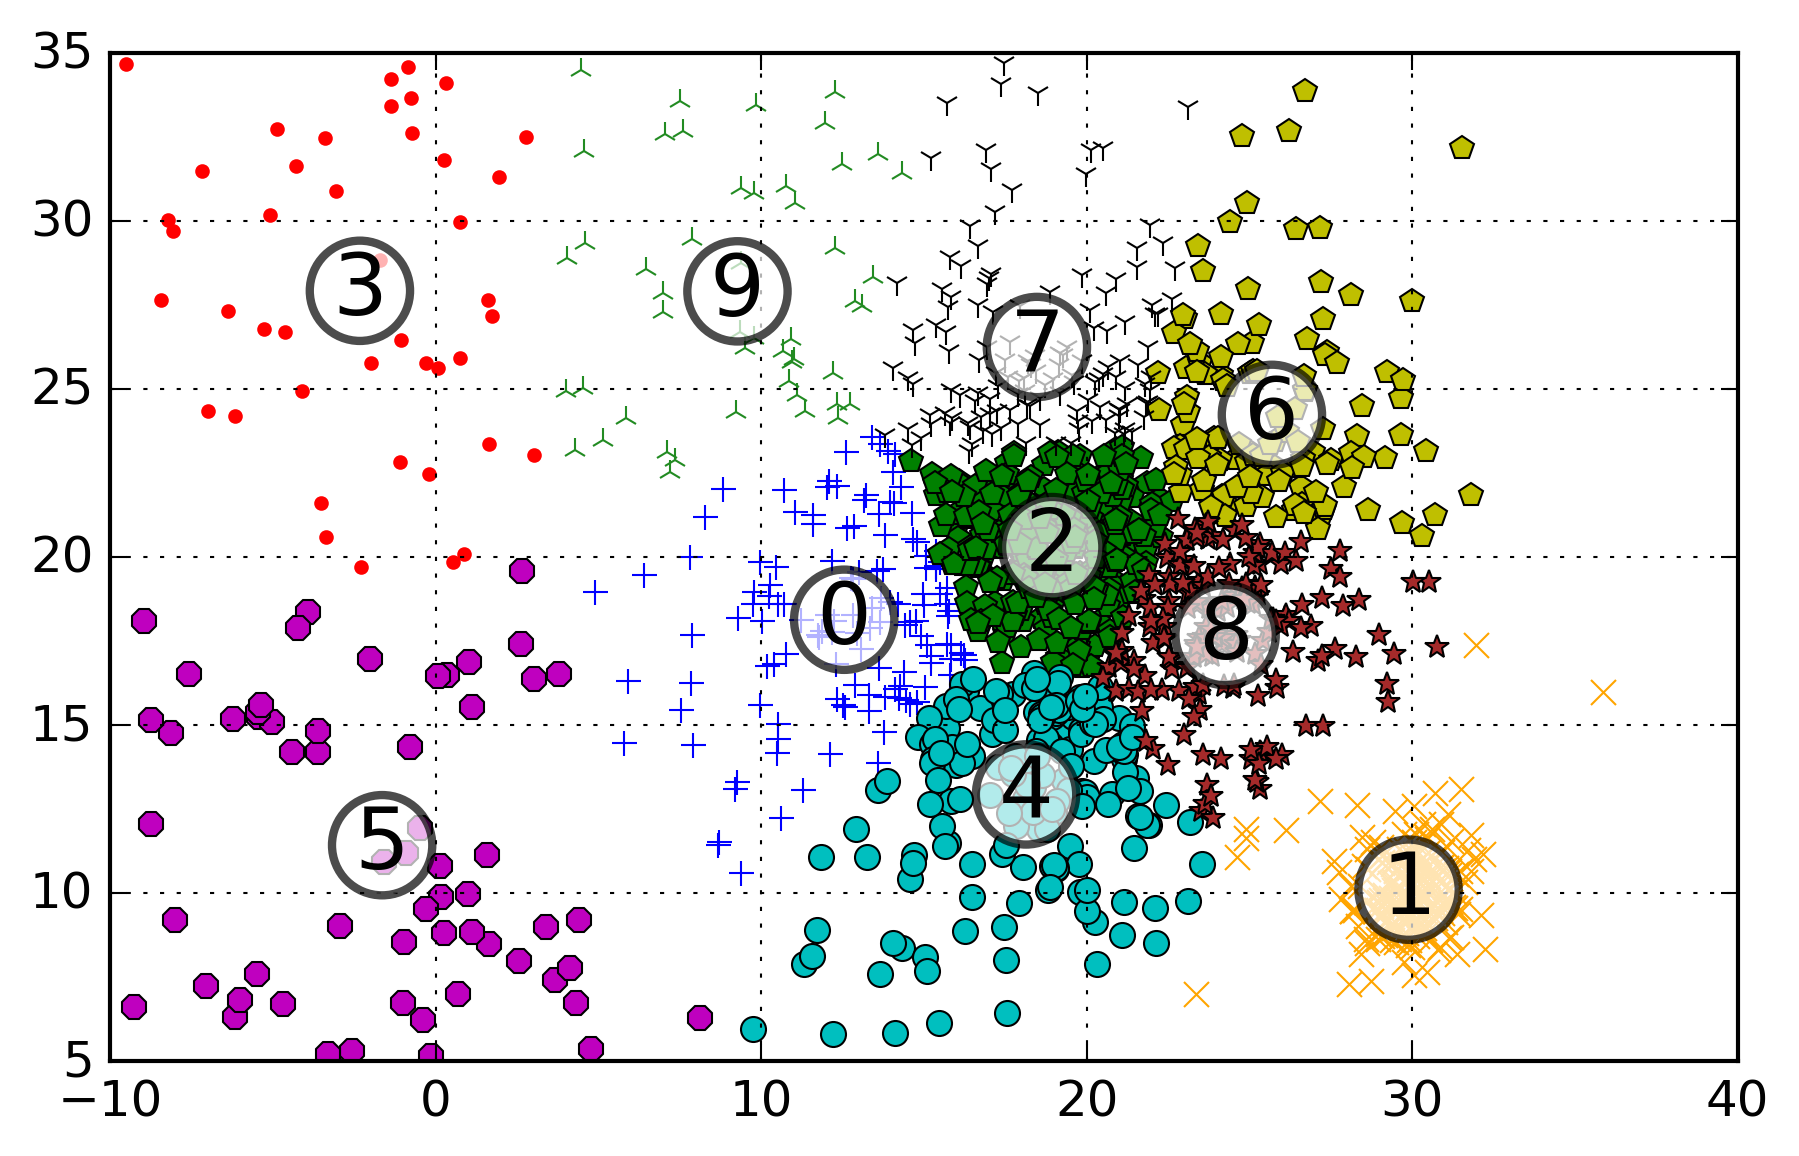
\includegraphics[width=\columnwidth]{img/adaptive_eta_without_threshold_ini.png}\label{fig_sub_eta_ini}} \\
   %\quad
   \subfloat[]
    {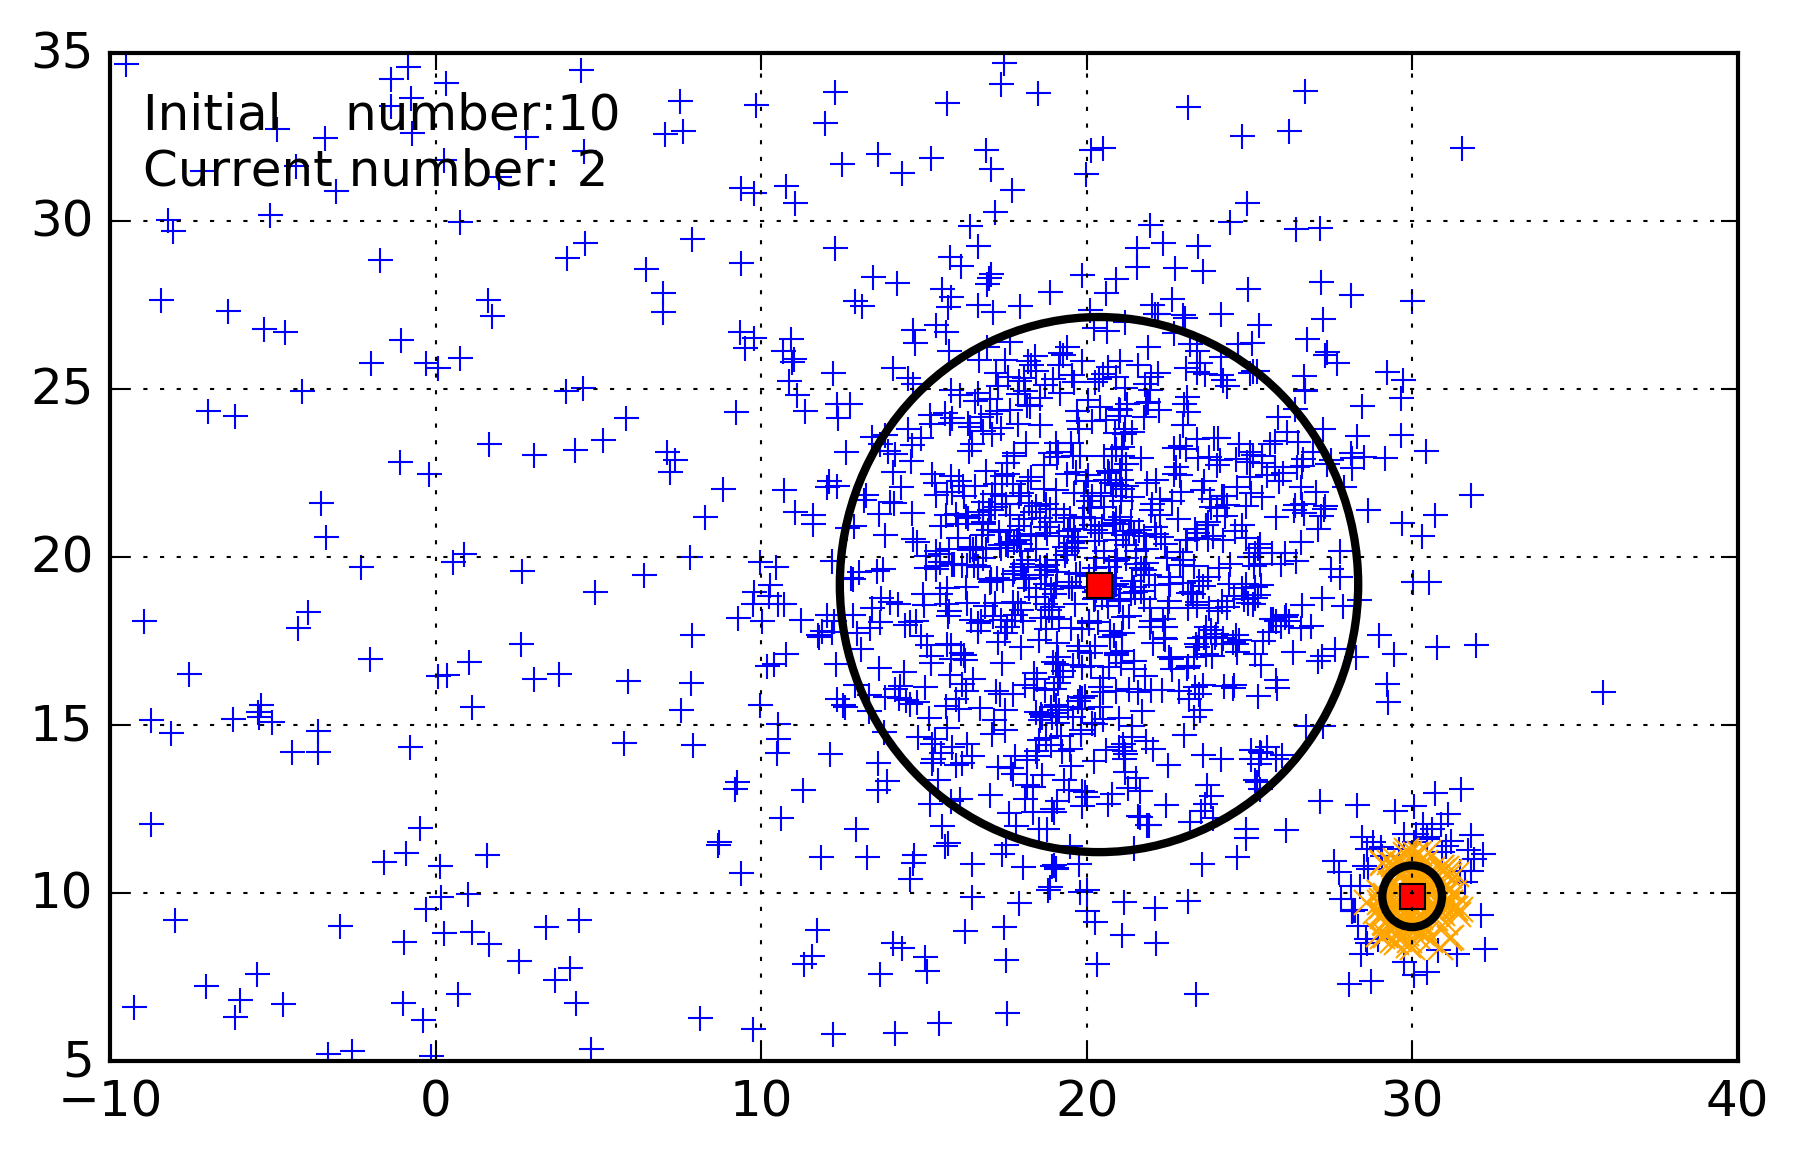
\includegraphics[width=\columnwidth]{img/adaptive_eta_without_threshold_last_frame.png}\label{fig_sub_eta_result}}
\caption{Detailed description of this dataset is in Experiment 1. (a) 10 initial partitions obtained by K-Means. (b) The $\eta$ of the large cluster is over-estimated because of the noisy points on the left, whereas the $\eta$ of the small cluster is under-estimated. The radius of each circle is the corresponding $\eta_j$}
\label{fig_eta}
\end{figure}

From the previous analysis, the NPCM algorithm is summarized in Algorithm \ref{alg:npcm}.
\begin{algorithm}
\caption{ [$\Theta$, $U$, $label$] = NPCM($X$, $m_{ini}$, $\alpha$)}
\label{alg:npcm}
\begin{algorithmic}[1]
\Require {$X$, $m_{ini}$, $\alpha$}
\State $m=m_{ini}$
\State \textbf{Set:} $\alpha=10^{-5}$ if $\alpha==0$
\State \textbf{Set:} $\alpha=1-10^{-5}$ if $\alpha==1$
\Statex {\Comment {Initialization and possible noise cluster elimination}}
\State Run K-Means.
\State Initialize $\theta_j$ and $\eta_j$ via \eqref{npcm_ini_theta} and \eqref{npcm_ini_eta}
\State Caculate $\rho_j$ via \eqref{npcm_density}
\State \textbf{Set:} $\rho_0=\max_j\rho_j$
\State Cluster $j$ is eliminated if $\rho_j<0.1\rho_0$
\State \textbf{Set:} $m=m-p$ if $p$ clusters are eliminated
\Repeat
\State Update $U$ via \eqref{npcm_u_update}
\State Update $\Theta$ via \eqref{upcm_theta_update}
\Statex {\Comment {Possible cluster elimination}}
\For{$i \leftarrow 1 \textbf{ to } N$}
\State \textbf{Set:} $label(i)=r$ if $u_{ir}=\max_j u_{ij}$
\EndFor
\State Cluster $j$ is eliminated if $j \notin label$
\State \textbf{Set:} $m=m-p$ if  $p$ clusters are eliminated
\Statex {\Comment {Bandwidth update and possible cluster elimination}}
\State Update $\eta_j$ via \eqref{npcm_eta_update}
\State Cluster $j$ is eliminated if $\eta_j=0$ (This happens if there is only one point in cluster $j$)
\State \textbf{Set:} $m=m-p$ if  $p$ clusters are eliminated
\Until{the change in $\theta_j$'s between two successive iterations becomes sufficiently small}\\
\Return {$\Theta$, $U$, $label$}
\end{algorithmic}
\end{algorithm}
\section{Experimental Results}
\label{sec-4}
In this section, we investigate the flexibility of choosing parameters in NPCM and also the benefit of the noise level parameter $\alpha$ through experiments. For the experiments of this paper, the algorithm terminates when the change in $\theta_j\text{s}$ between two successive iterations is below than $10^{-5}$, i.e., $\Sigma_j\|\boldsymbol{\theta}_j^{t}-\boldsymbol{\theta}_j^{t-1}\|\leq10^{-5}$. The circle centers of all figures are the corresponding $\boldsymbol{\theta}_j\text{s}$.

\textbf{Experiment 1:} In this dataset, there are two physical clusters generated by normal distributions with centers $\mathbf{c_1}=[20, 20]^T$, $\mathbf{c_2}=[30, 30]^T$, covariance matrixes $\mathbf{\Sigma_1}=20\mathbf{I}$, $\mathbf{\Sigma_2}=\mathbf{I}$, $N_1=1000$ points, and $N_2=200$ points  respectively, where $\mathbf{I}$ is the $2\times 2$ identity matrix. Moreover, 200 data points are added randomly as noise in the region where data live. 
The initialization result obtained by K-Means with 10 clusters is shown in Fig.\ref{fig_sub_eta_ini}.

In order to show the parameter-choosing flexibility, we run NPCM with $m_{ini}=10$ and several $\alpha\text{s}$. The result is shown in Fig.\ref{fig_small_cluster}.
We can see that the small cluster is identified correctly when there is a large cluster near it. Furthermore, the clustering result and the estimated $\eta_j\text{s}$ are not sensitive to the choosing of $\alpha$ for this dataset. 
\begin{figure*}[tb]
\captionsetup[subfloat]{farskip=1pt,captionskip=1pt}% use this to reduce space between rows of subfloats, or between subfloat and the caption
   \centering
   \subfloat[]
    {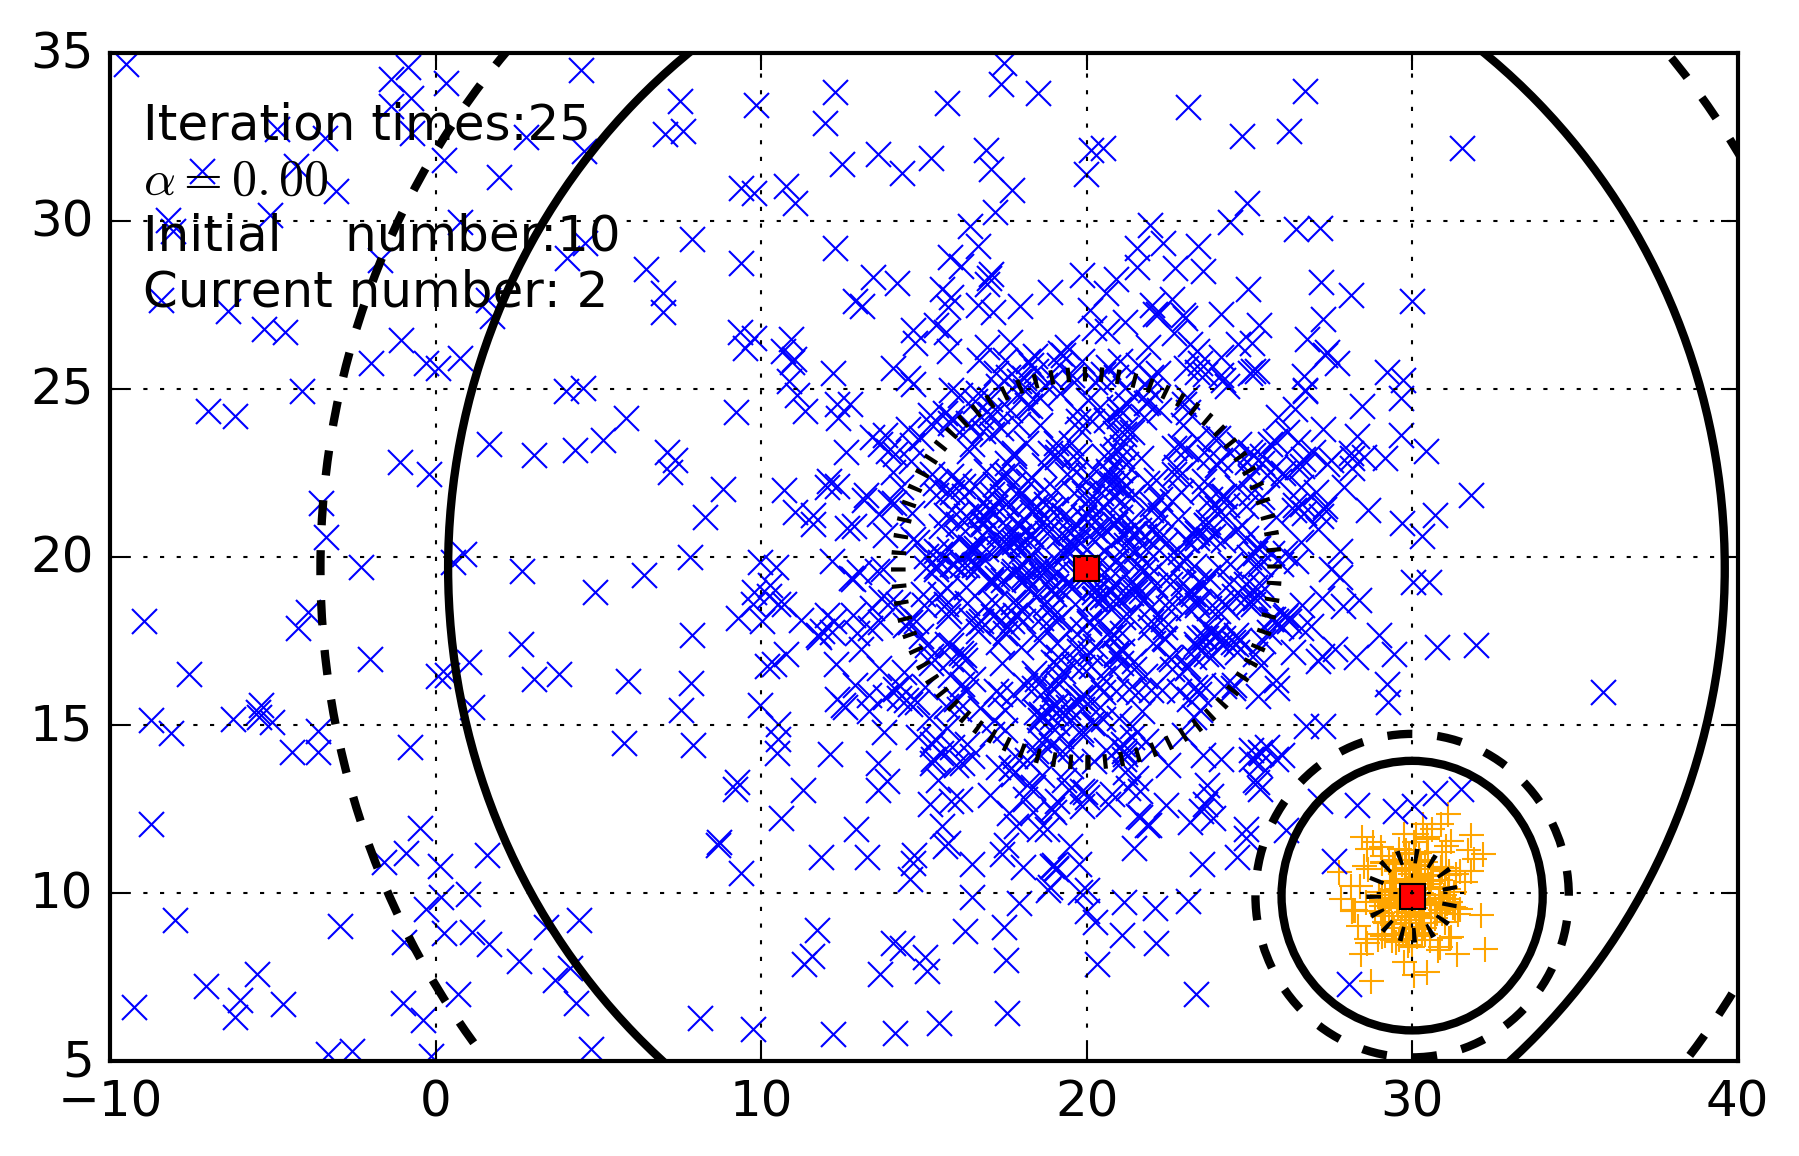
\includegraphics[width=\columnwidth]{img/small_cluster_structure_preserve_last_frame_n_10_alpha_0_0.png}\label{fig_sub_small_0}}
   \quad
   \subfloat[]
    {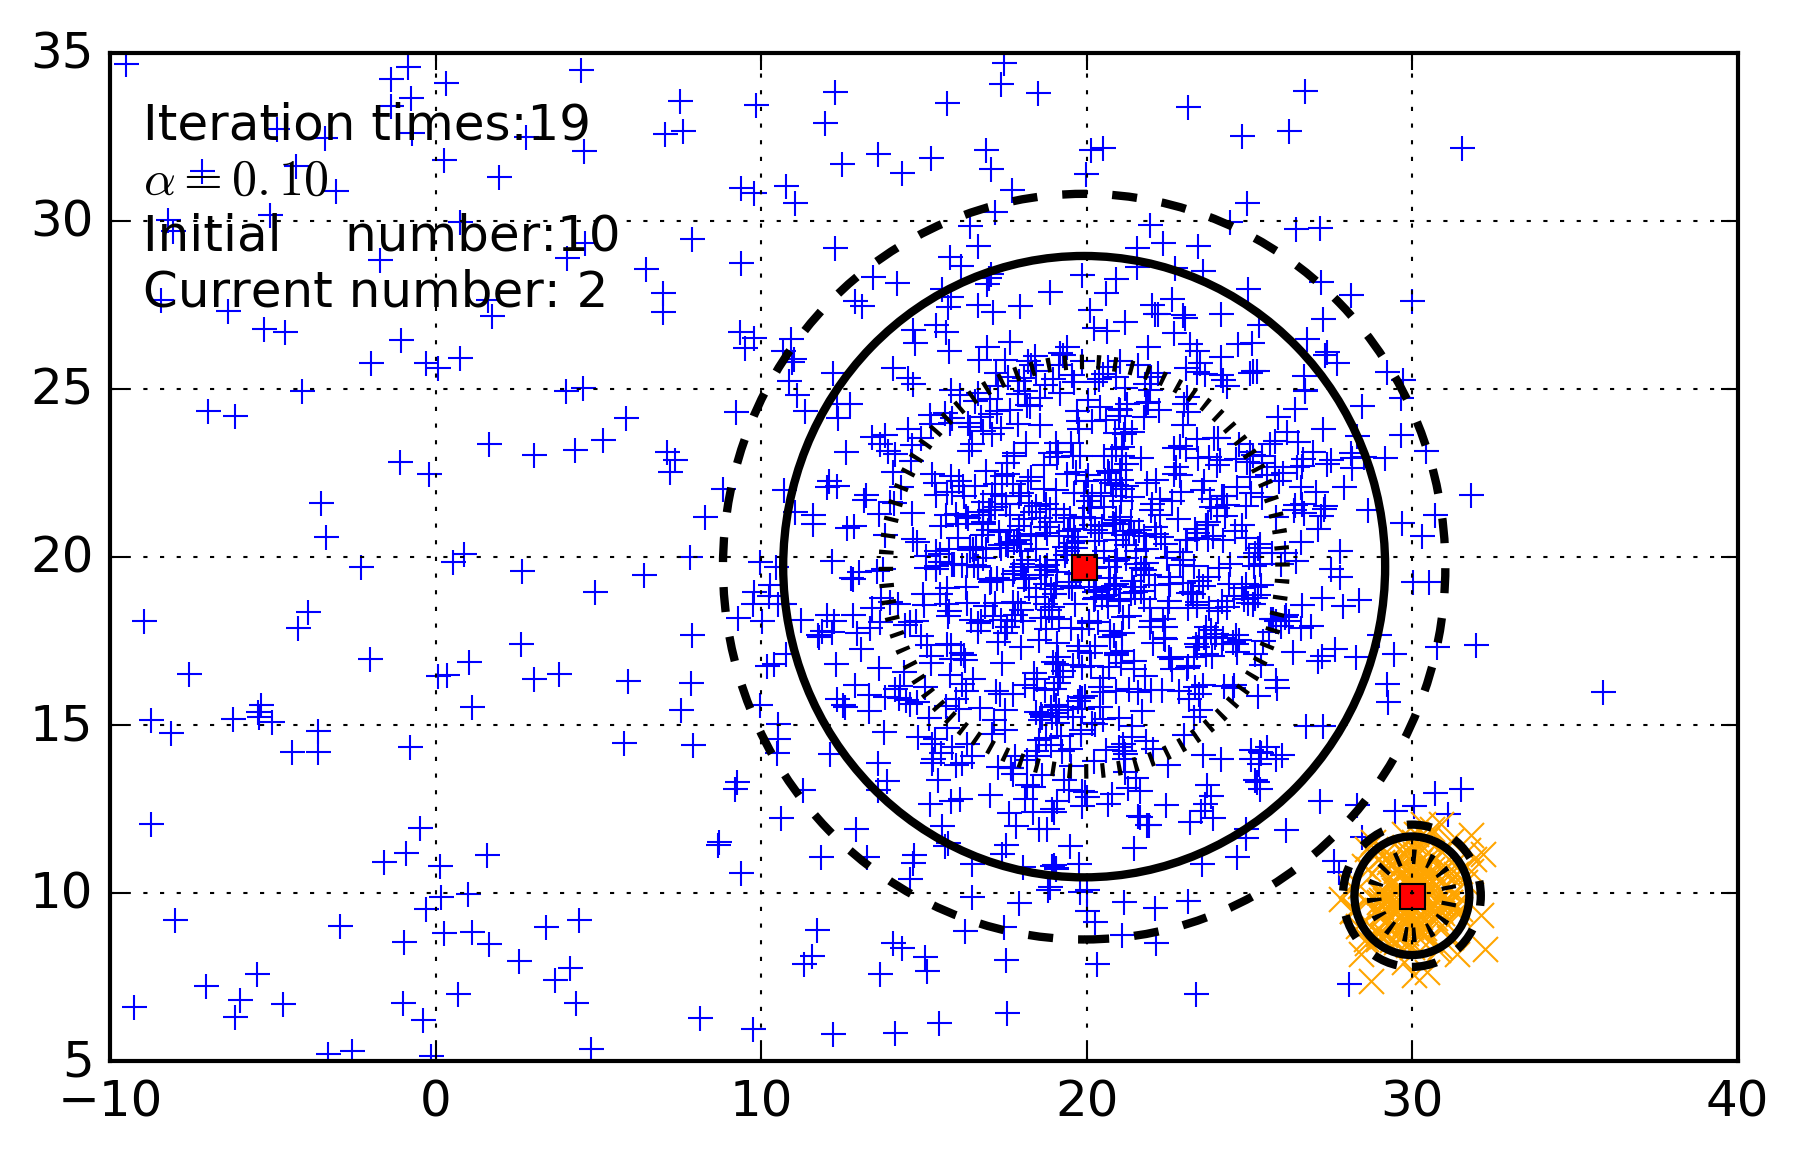
\includegraphics[width=\columnwidth]{img/small_cluster_structure_preserve_last_frame_n_10_alpha_0_1.png}\label{fig_sub_small_0_1}} \\
    \subfloat[]
    {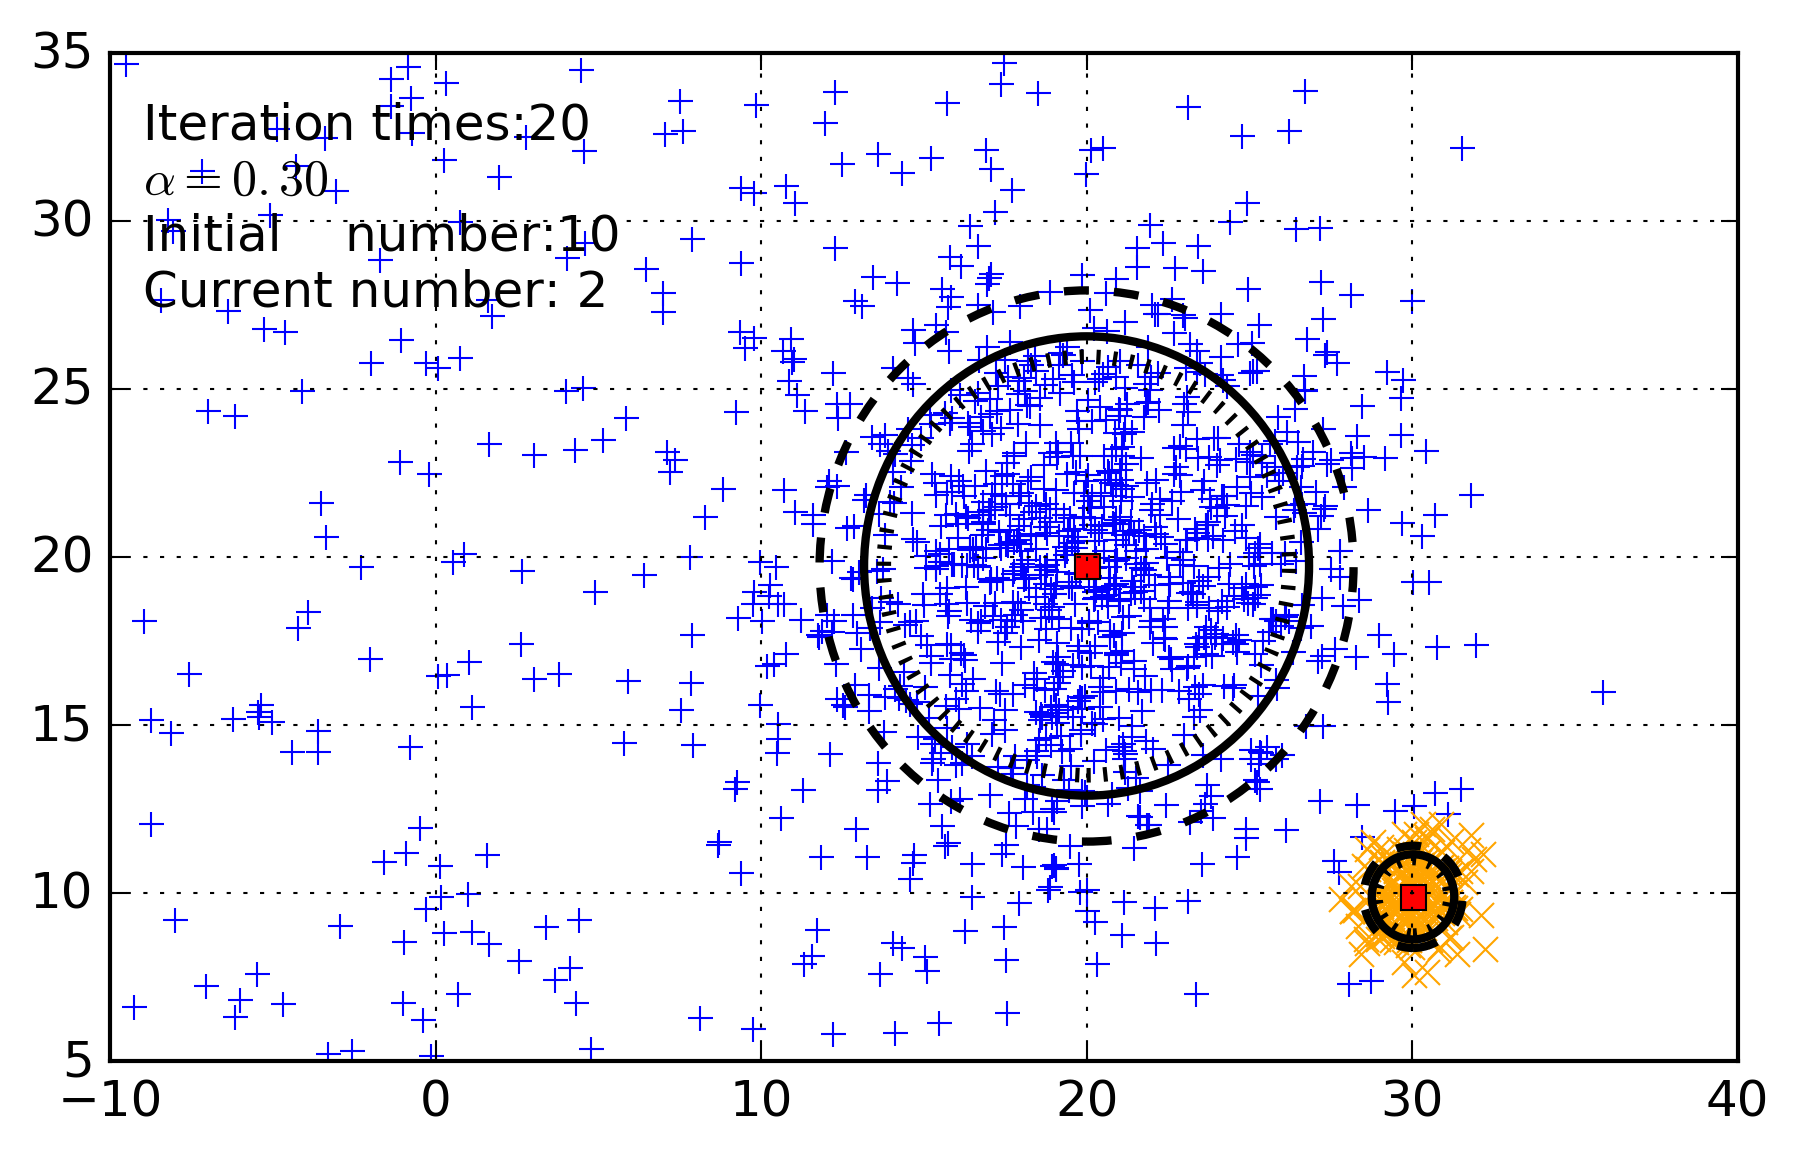
\includegraphics[width=\columnwidth]{img/small_cluster_structure_preserve_last_frame_n_10_alpha_0_3.png}\label{fig_sub_small_0_3}}
   \quad
   \subfloat[]
    {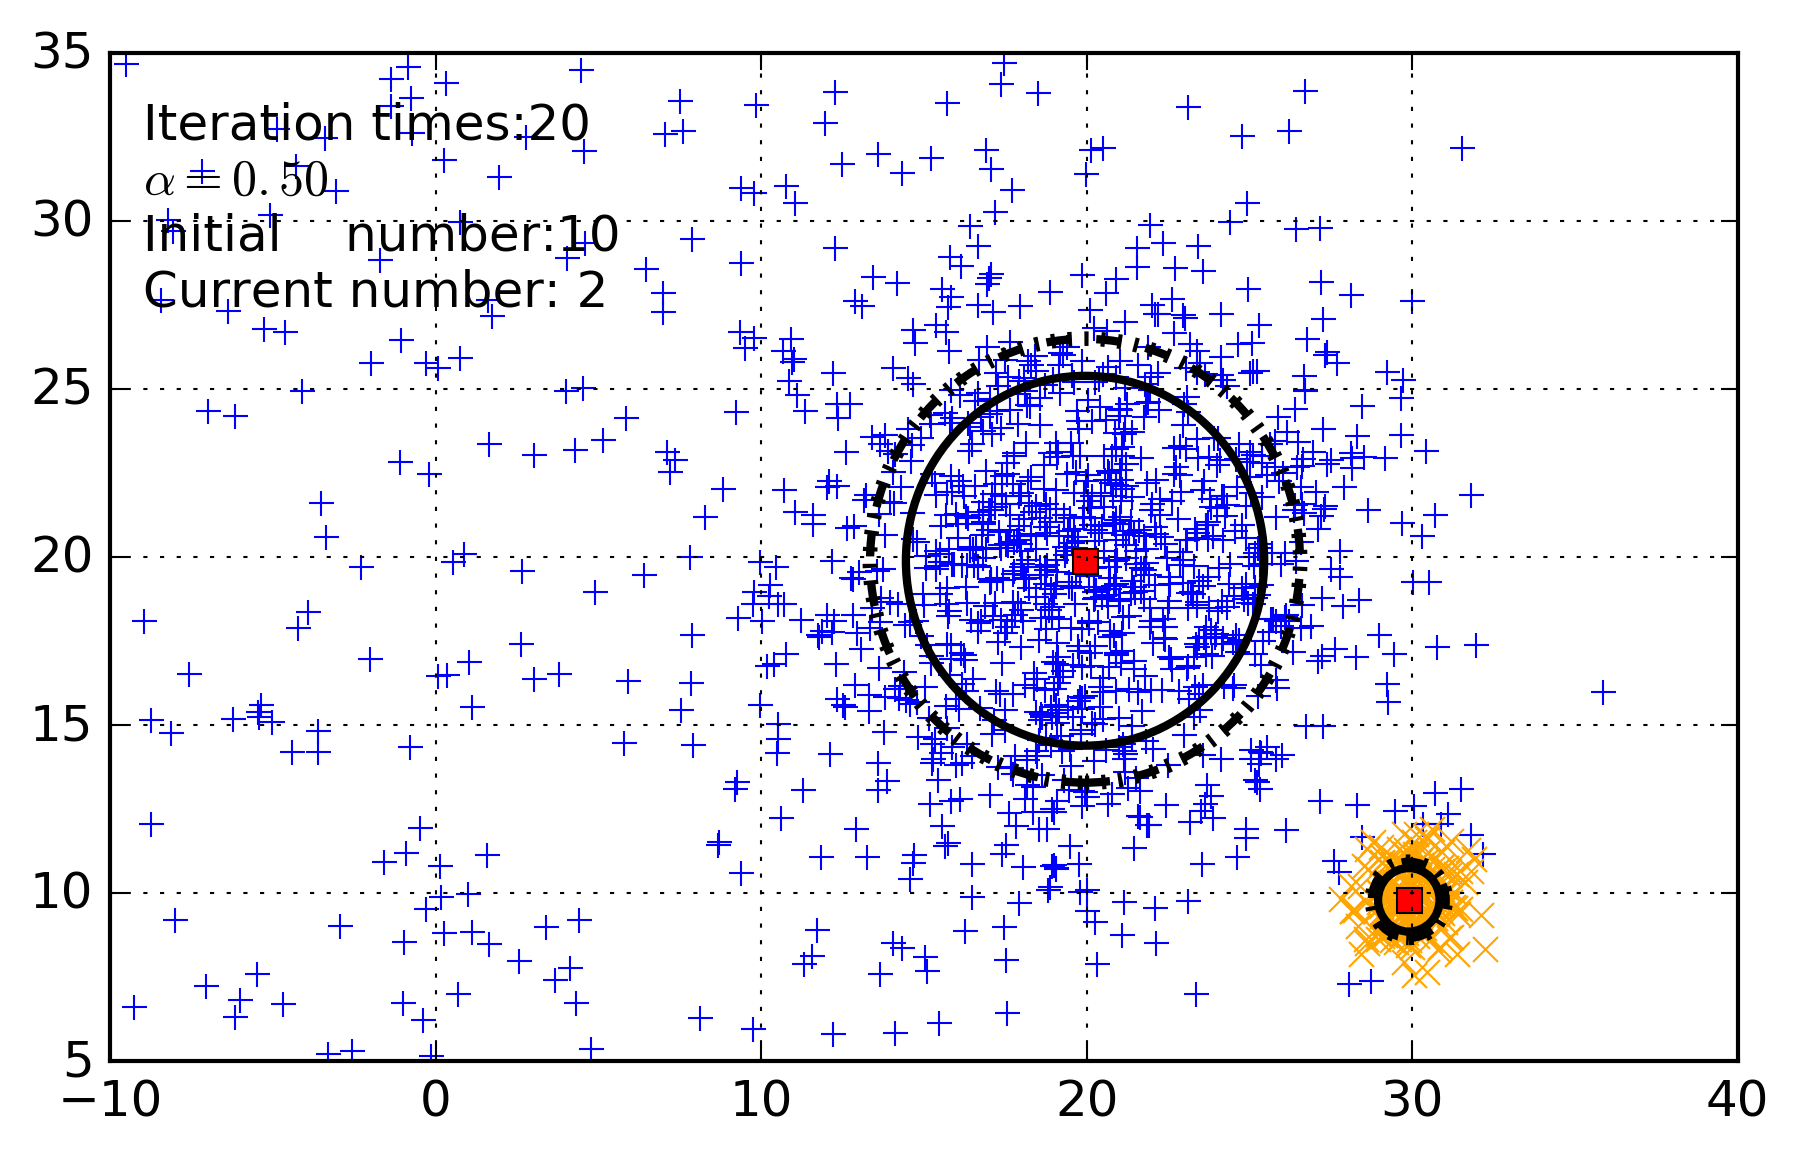
\includegraphics[width=\columnwidth]{img/small_cluster_structure_preserve_last_frame_n_10_alpha_0_5.png}\label{fig_sub_small_0_5}}
\caption{The clustering result of NPCM with $m_{ini}=10$, (a) $\alpha=0$, (b) $\alpha=0.1.$ (c) $\alpha=0.3$, (d) $\alpha=0.5$.
The circles with radius $\eta_j$, $d_{j\alpha}^0$, and $d_{j\alpha}$ are represented by the dotted circle, solid circle, and dashed circle, respectively (e.g., in (a), the inner circle, middle circle, and the outer circle respectively).}
\label{fig_small_cluster}
\end{figure*}

In the next experiment, we investigate a situation where the parameter $\alpha$ matters.

\textbf{Experiment 2:} In this dataset, there are two overlapped physical clusters generated by normal distributions with centers $\mathbf{c_1}=[2.25, 1.5]^T$, $\mathbf{c_2}=[1.9, 1.9]^T$, covariance matrixes $\mathbf{\Sigma_1}=0.2^2\mathbf{I}$, $\mathbf{\Sigma_2}=0.2^2\mathbf{I}$, $N_1=400$ points, and $N_2=400$ points  respectively. The dataset is shown in Fig.\ref{fig_sub_close_ori}.

NPCM is run with $m_{ini}=10$ and several $\alpha\text{s}$. The result is shown in Fig.\ref{fig_close_cluster}. In Fig.\ref{fig_sub_close_0_1}, the two clusters merge due to the specification of a small noise level parameter $\alpha=0.1$. In Fig.\ref{fig_sub_close_0_3}, when $\alpha$ increase to $0.3$, the generated clusters overlap with each other just as the physical clusters. In Fig.\ref{fig_sub_close_0_5}, when $\alpha=0.5$, the influence of points in other clusters can be effectively reduced, so we get two well-separated clusters. 
\begin{figure}[tb]
\captionsetup[subfloat]{farskip=1pt,captionskip=1pt}% use this to reduce space between rows of subfloats, or between subfloat and the caption
   \centering
   \subfloat[]
    {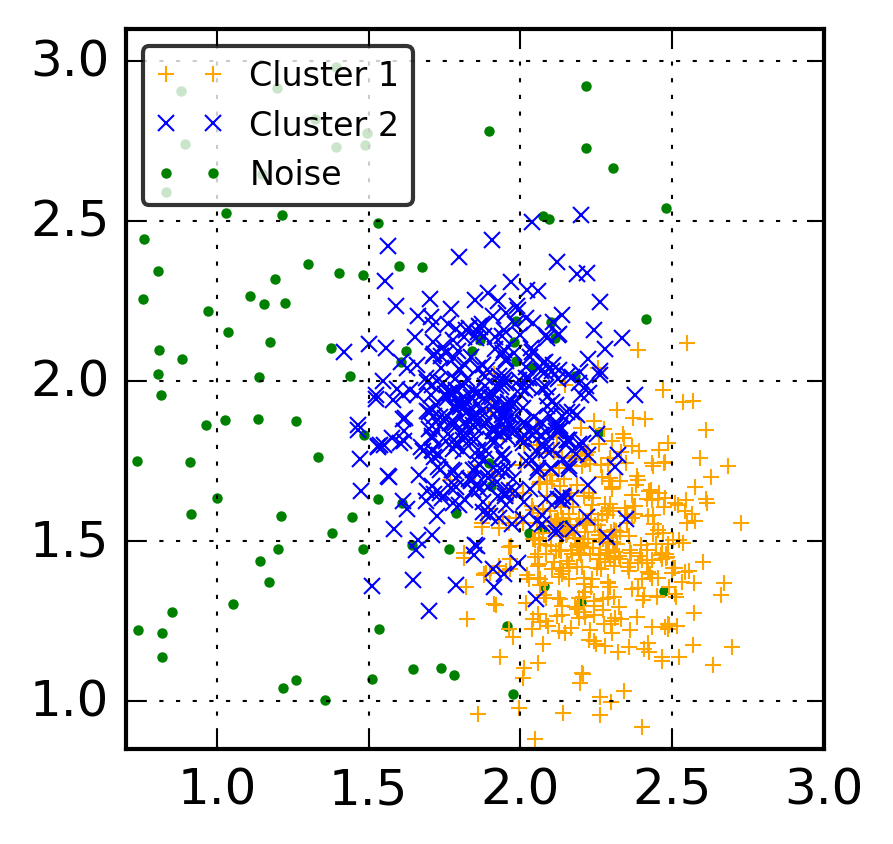
\includegraphics[width=0.5\columnwidth]{img/example_close_cluster_ori.png}\label{fig_sub_close_ori}}
   %\quad
   \subfloat[]
    {\includegraphics[width=0.5\columnwidth]{img/example_close_cluster_last_frame_n_10_alpha_0_1.png}\label{fig_sub_close_0_1}} \\
    \subfloat[]
    {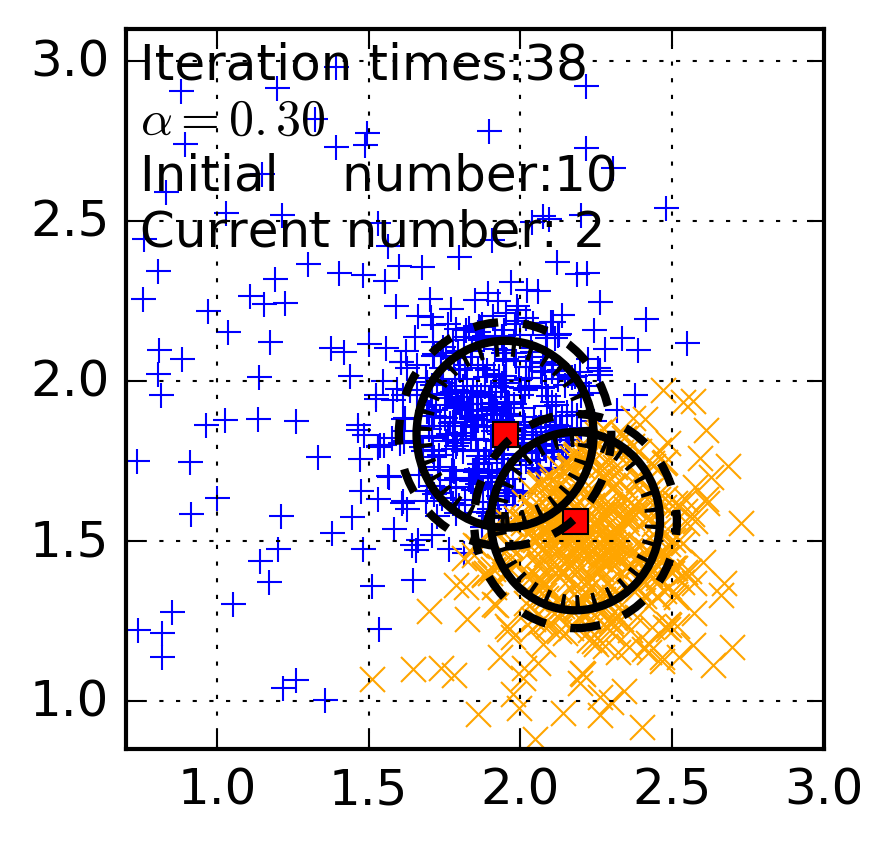
\includegraphics[width=0.5\columnwidth]{img/example_close_cluster_last_frame_n_10_alpha_0_3.png}\label{fig_sub_close_0_3}}
   %\quad
   \subfloat[]
    {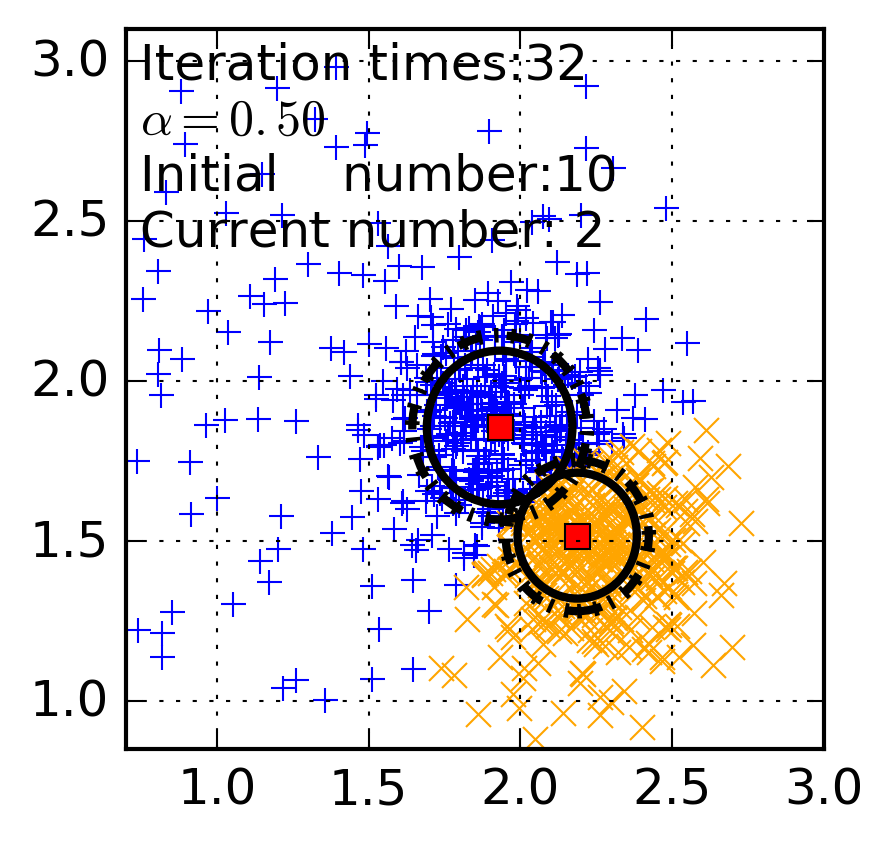
\includegraphics[width=0.5\columnwidth]{img/example_close_cluster_last_frame_n_10_alpha_0_5.png}\label{fig_sub_close_0_5}}
\caption{(a) Dataset of experiment 2. The clustering result of NPCM with $m_{ini}=10$, (b) $\alpha=0.1.$, (c) $\alpha=0.3$, and (d) $\alpha=0.5$.
The radius of each circle is of the same meaning as in Fig.\ref{fig_small_cluster}.}
\label{fig_close_cluster}
\end{figure}

In summary, the parameter $\alpha$ should be chosen to  properly characterize the closeness of clusters in the clustering result. Specifically, if we specify a low noise level, e.g., in Experiment 2, $\alpha=0.1$, but the true noise level of the physical clusters is higher (i.e., they are closer to each other than we think), then NPCM would treat them as one cluster and the clusters merge; in Experiment 1, there are no overlapped clusters, and we can set an arbitrary $\alpha$.
However, as pointed out in UPCM, each physical cluster can be seen as noise to other physical clusters. So we should specify a large noise level $\alpha$ in order to robustly characterize the closeness of clusters in the dataset (i.e., noise level of the dataset).
\section{Conclusion}
\label{sec-5}
In this paper, we develop a noise level based PCM clustering algorithm (NPCM). Specifically, NPCM addresses the background noise cluster problem encountered in APCM and UPCM and exploit the intuition from UPCM to eliminate the parameter $\sigma_v$ based on $\eta_j$.
There are two parameters in NPCM: $m_{ini}$ is a possibly over-specified number of clusters to ensure that there is at least one cluster placed near each physical cluster in the initial partition, and $\alpha$ characterizes the closeness of clusters in the clustering result.
The advantage of NPCM is that the parameter $\alpha$ is intuitive to choose and NPCM does not need strong prior information (e.g., the exact cluster number or the exact closeness of clusters) of the dataset.
Furthermore, we find that the update of $\eta_j$ is a positive feedback process and the adaptive $\sigma_v$ mechanism adopted in NPCM makes this positive feedback process more stronger, and a direct consequence of this fact is that NPCM has a faster convergence rate. 
Experiments show that the clustering result is not sensitive to the choosing of $\alpha$ unless there are overlapped clusters in the dataset.
In addition, the Appendix shows the convergence behavior of NPCM.
\appendix
In this appendix, we prove the cluster elimination and the convergence of the prototypes to the center of dense regions. Because some convergence results of APCM \cite{xenaki_novel_2016} are applicable to NPCM, we only give the essential part of the proof. 

We consider the continuous case where data points are modeled by a random variable $\mathbf{x}$ that follows a continuous pdf distribution $p(\mathbf{x})$. In this case, the update equations are given below:
\begin{equation}
\boldsymbol{\theta}_j^{t+1}=\frac{\int_{R_j^t} u_{j}^t(\mathbf{x})\mathbf{x}p(\mathbf{x})d\mathbf{x}}{\int_{R_j^t} u_{j}^t(\mathbf{x})p(\mathbf{x})d\mathbf{x}} 
\end{equation}
where $R_j^t=\{\mathbf{x}|u_{j}^t(\mathbf{x}) \geq \alpha\}$,
\begin{IEEEeqnarray}{ll}
u_{j}^t(\mathbf{x}) &= \exp\left(\frac{||\mathbf{x}-\boldsymbol{\theta}_j^t||^2}{\gamma_j^t}\right) \\
\gamma_j^t &= \left(0.5\eta_{j}+0.5\sqrt{\eta_{j}^{2}+0.8d_{j}\eta_j/\sqrt{-\ln\alpha}}\right)^2
\end{IEEEeqnarray}
and 
\begin{equation}
\eta_{j} = \frac{\int_{T_j^{t}} ||\mathbf{x}-\boldsymbol{\theta}_j^{t}||p(\mathbf{x})d\mathbf{x}}{\int_{T_j^{t}} p(\mathbf{x})d\mathbf{x}}
\end{equation}
with $T_j^{t}=\{\mathbf{x}|u_{j}^{t}(\mathbf{x})=\max_r u_{r}^{t}(\mathbf{x}), u_{j}^t(\mathbf{x}) \geq 0.01\}$.

The above equations define the iterative scheme $\boldsymbol{\theta}_j^{t+1}=f(\boldsymbol{\theta}_j^{t})$, where
\begin{equation}
\label{npcm_iteration_scheme}
f(\boldsymbol{\theta}_j^t)=\frac{\int_{R_j^t} \exp\left(-\frac{\|\mathbf{x}-\boldsymbol{\theta}_j^t\|^2}{\gamma_j^t}\right)\mathbf{x}p(\mathbf{x})d\mathbf{x}}{\int_{R_j^t} \exp\left(-\frac{\|\mathbf{x}-\boldsymbol{\theta}_j^t\|^2}{\gamma_j^t}\right)p(\mathbf{x})d\mathbf{x}} 
\end{equation}


\begin{prop}
Assume that $p(\mathbf{x})$ is a zero mean normal distribution ${\cal N}(\mathbf{0},\sigma^2I)$. Then the center $\mathbf{c}=\mathbf{0}$ of $p(\mathbf{x})$ is a fixed point for the iterative scheme defined by \eqref{npcm_iteration_scheme}. Furthermore, the fixed point $\mathbf{0}$ of the scheme $\boldsymbol{\theta}^{t+1}=f(\boldsymbol{\theta}^{t})$ is stable.
\label{prop_fix_stable}
\end{prop}

\begin{proof}
See the proof of Proposition 3 and Proposition 4 in \cite{xenaki_novel_2016}.
\end{proof}

In the general case where data form more than one dense regions, Proposition \ref{prop_fix_stable} is still valid, assuming that a proper $\alpha$ is specified so that the influence on a prototype that belongs to a given dense region from points from other dense regions is negligible.

\begin{prop}
Let $\boldsymbol{\theta}_1$, $\boldsymbol{\theta}_2$ be two cluster prototypes with $\eta_1>\eta_2$ in the same dense region. Then cluster $C_2$ represented by $\boldsymbol{\theta}_2$ will be eliminated.
\label{prop_eliminate}
\end{prop}

\begin{proof}
 We first calculate the geometrical locus of the points $\mathbf{x}$ having $u_2(\mathbf{x})>u_1(\mathbf{x})$, where $u_j(\mathbf{x})=\exp\left(-\frac{d_j^2(\mathbf{x})}{\gamma_j}\right)$ and $d_j(\mathbf{x})=\|\mathbf{x} - \boldsymbol{\theta}_j\|^2$, $j=1,2$.
From \eqref{npcm_d_alpha} and \eqref{npcm_sig_alpha_relation}, we get $d_{u_1}=\sqrt{-\ln u_1}\left(\eta_1+\sqrt{-\ln u_1}\sigma_{v_1}\right)=1.2\sqrt{-\ln u_1}\eta_1$ and $d_{u_2}=1.2\sqrt{-\ln u_2}\eta_2$, where we use $u_1$ and $u_2$ to represent $u_1(\mathbf{x})$ and $u_2(\mathbf{x})$ respectively. 

For the points $\mathbf{x}$ that meet $u_1<u_2$, we have 
\begin{equation*}
\frac{d_{u_1}}{d_{u_2}}=\frac{1.2\sqrt{-\ln u_1}\eta_1}{1.2\sqrt{-\ln u_2}\eta_2}>\frac{\eta_1}{\eta_2}(1+\epsilon)=k'>\frac{\eta_1}{\eta_2}=k>1
\end{equation*}
where $\epsilon\in(0,+\infty)$. Then we get $\|\mathbf{x} - \boldsymbol{\theta}_1\|^2 > k'\|\mathbf{x} - \boldsymbol{\theta}_2\|^2$, and we have after some algebra
\begin{equation}
\label{hypersphere}
\|\mathbf{x}-\frac{k'\boldsymbol{\theta}_2-\boldsymbol{\theta}_1}{k'-1}\|^2 = \frac{k'}{(k'-1)^2}\|\boldsymbol{\theta}_2-\boldsymbol{\theta}_1\|^2\equiv r^2
\end{equation}

Utilizing Proposition \ref{prop_fix_stable}, we have that $\boldsymbol{\theta}_1$ and $\boldsymbol{\theta}_2$ converge towards $\mathbf{c}$. Thus, the distance between them decreases towards zero, i.e., 
\begin{equation}
\|\boldsymbol{\theta}_1(t)-\boldsymbol{\theta}_2(t)\|\rightarrow 0
\label{eqprop51}
\end{equation}          

So the radius $r$ in \eqref{hypersphere} tends to zero as $t$ increases, which means that there will be no points in cluster $C_2$ and $C_2$ will be eliminated.

Note that $k'$ is larger than the $k$ used in the proof of APCM, so convergence of NPCM is faster than APCM. 
See the proof of Proposition 2 and Proposition 5 in \cite{xenaki_novel_2016} for details.
\end{proof}




\bibliographystyle{IEEEtran}
\bibliography{D:/emacs/etc/ZoteroOutput,IEEEabrv}
% Emacs 24.5.1 (Org mode 8.2.10)
\end{document}
